
\subsection{Klassen und ihre Funktionen}
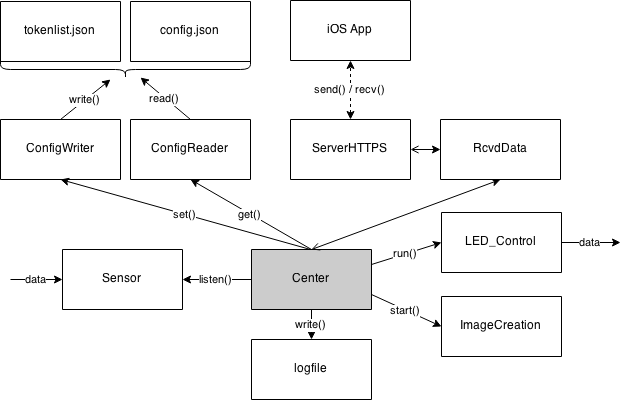
\includegraphics[width=1 \textwidth]{./data/ApplicationConcept.png}{\centering}
\begin{itemize}
\item Center\\
Die Klasse 'Center' stellt die zentrale Stelle in der Anwendung dar, an der alle Informationen zusammen laufen und verwaltet werden.
\item ServerHTTPS\\
Hier läuft der Webserver, welcher Nachrichten empfängt und sendet. Empfangene Nachrichten werden an die Klasse 'RcvdData' übergeben.
\item RcvdData\\
Hier werden die empfangenen Nachrichten ausgewertet und entsprechende Antworten generiert. Diese werden an den Webserver zurück gegeben und abgesendet. Die Prüfung der Korrektheit der einzelnen Protokollbestandteile findet ebenfalls hier statt. Wenn alle Überprüfungen erfolgreich sind, werden die Befehle an 'Center' weiter gegeben und dort ausgeführt.
\item Sensor\\
In der Klasse 'Sensor' werden die einzelnen Bewegungssensoren überwacht. Falls eine Bewegung detektiert wird, so werden in 'Center' die notwendigen Methoden aufgerufen um die LEDs an- oder auszuschalten.
\item LED-Control\\
Die Klasse 'LED\_Control' verwaltet die eingerichteten LEDs und steuert diese. Hier werden auch die möglichen Effekte gesteuert. Die Methoden in dieser Klasse werden aus der Klasse 'Center' aufgerufen. Ein Zugriff in die andere Richtung ist nicht möglich.
\item ConfigReader / ConfigWriter\
Diese beiden Klassen bieten die Möglichkeit die Konfigurationsdatei config.json zu lesen und zu schreiben. In der Konfiguration werden Informationen wie Anzahl der LEDs, Passworthash oder Adresse der Netzwerkkamera abgespeichert. Die Konfigurationsdatei wird beim Installationsvorgang erstellt.
\item Cam\\
Abrufen von Bildmaterial von der Netzwerkkamera oder vom Server findet ausschließlich über die Klasse 'Cam' statt. Die Klasse ruft die Informationen ab und filtert das Bildmaterial.
\item UNIT-Test\\
Einzelne Rückgabetypen von Methoden, sowie die Initialisierung von allen Klassen kann mit 'UNIT\_Test' getestet werden.
\item Logfile\\
Im Logfile werden unter anderem auftretende Fehler gespeichert.
\end{itemize}

\subsection{Auswertung empfangener Daten}
Da die Daten anhand des ausgearbeiteten Protokolls übertragen werden, können sie als String sehr einfach an den ":" aufgesplittet werden. Im Anschluss werden sie einzelnen Variablen zugewissen (bessere Lesbarkeit des Codes). Bevor das 'Control'-Feld ausgewertet wird, muss der Hashwert der Übertragung und die Authentifizierung geprüft werden. 

\begin{lstlisting}[caption=Auswertung der empfangenen Daten (RcvdData.py), language=python, frame=single, breaklines=true,columns=fullflexible, commentstyle=\color{gray}\upshape, captionpos=b, numbers = left]
class RecvdData(threading.Thread):
    def dataReceived(self, data):
        # Protokoll: auth:pw:control:ledNo:rangeStart:rangeEnd:red:green:blue:modus:effectcode:config:hashv
        # Beispiel: admin:w:X00:1:0:0:10:10:10:0:0:w-w:58acb7acccce58ffa8b953b12b5a7702bd42dae441c1ad85057fa70b
        a = data.split(':')
        if len(a) > 1:
            auth = 		a[0]
            pw = 		a[1]
            control = 	a[2]
            ledNo = 	a[3]
            rangeStart = a[4]
            rangeEnd = 	a[5]
            red = 		a[6]
            green = 	a[7]
            blue = 		a[8]
            modus = 	a[9]
            effectcode = a[10]
            config = a[11]
            hashv = a[12]
            data = auth + pw + control + ledNo + rangeStart + rangeEnd + red + green + blue + modus + effectcode + config
            data = data.rstrip('\n')
            data = data.rstrip('\r')
            if (self.checkAuthentification(auth, pw) & self.checkTransmissionData(data, hashv)):
                if control == 'X00':
                    ## Alle LEDs ausschalten
                    center.clearPixel()
                elif control == 'X01':
                    ## Eine LED anschalten
                    self.lightUpOneLED(int(ledNo), int(red), int(green), int(blue))
                elif control == 'X02':
                    ## LED Bereich anschalten
                    self.lightUpLEDRange(int(rangeStart), int(rangeEnd), int(red), int(green), int(blue))
                elif control == 'X03':
                    ## Eine Farbe für alle LED
                    self.lightUpAllLED(int(red), int(green), int(blue))
                elif control == 'X04':
                    ## Effekt alle LEDs
                    self.effectLED(effectcode)
                elif control == 'X05':
                    ## Modus des Systems
                    self.changeModus(int(modus))
                elif control == 'X06':
                    ## Systemstatus als JSON an den Client
                    return self.sendStatus()
                elif control == 'X07':
                    ## Status der einzelnen LEDs senden
                    return self.sendLEDStatus()
                elif control == 'X08':
                    ## Konfiguration ändern
                    self.changeConfiguration(config)
                elif control == 'X09':
                    ## Login
                    return "LOGIN:TRUE"
            else:
                print center.writeLog('Übertragung fehlerhaft')
\end{lstlisting}
Die komplette Klasse ist einsehbar unter: https://github.com/hoedding/Studienarbeit-Anwendung/blob/master/RaspberryPI/RecvdData.py

\subsection{Konfiguration}
\paragraph{Konfigurations-Datei}
Die Informationen die zum Betrieb notwendig sind, werden in JSON-Format gespeichert.
\begin{lstlisting}[caption=Konfigurationsdatei config.json, language=json, frame=single, breaklines=true,columns=fullflexible, commentstyle=\color{gray}\upshape, captionpos=b, numbers = left]
{
  // Anzahl der LEDs
  "ledcount": "2",
  // Name des Benutzers
  "username": "testuser",
  // Hash des Nutzerpassworts
  "passhash": "58acb7acccce58ffa8b953b12b5a7702bd42dae441c1ad85057fa70b",
  // Port an dem ein Bewegungssensor angeschlossen wird
  "motionport1": "7",
  "motionport2": "8",
  // Verfügbarkeit der Netzwerkkamera
  "camavaible": "1",
  // URL der Kamera
  "cam_url": "test.de",
  "cam_url_short": "test2.de",
  // Zeitdauer der LED-Beleuchtung
  "timeperiod": "10",
  // FTP Details
  "ftp_url": "test3.de",
  "ftp_directory":"", 
   "ftp_user":"", 
   "ftp_pw":""
}
\end{lstlisting}
Diese Informationen können auch vom Client abgerufen werden: 
\begin{lstlisting}[caption=Senden von Konfigurationsinformationen an den Client, language=json, frame=single, breaklines=true,columns=fullflexible, commentstyle=\color{gray}\upshape, captionpos=b, numbers = left]
    def sendStatus(self):
        # Status des Systems senden
        reader = ConfigReader()
        message = 'STATUS:{"ledcount":"' + reader.getNumberOfLED() + '","motionport1":"' + reader.getMotionPin1() + '","motionport2":"' + reader.getMotionPin2() + '","ftp_url":"' + reader.getFTP() + '","camavaible":"'
        message = message + reader.camAvaible() + '","cam_url":"' + reader.camURL() + '","cam_url_short":"' + reader.camShortURL() + '","timeperiod":"' + reader.getTimePeriod() + '"}'
        return str(message)
\end{lstlisting}

\paragraph{Status der LED} Es ist möglich der Status der einzelnen LEDs abzurufen. Hierfür wird ein JSON-Objekt generiert, welches die einzelnen Farben als 24Bit-Werte enthält.
\begin{lstlisting}[caption=Status der LEDs an Client senden, language=json, frame=single, breaklines=true,columns=fullflexible, commentstyle=\color{gray}\upshape, captionpos=b, numbers = left]
  def getLEDStatusAsJson(self):
    led_values = led.getLedAsArray()
    data = 'LED:{"led": ['
    if len(led_values) > 0:
        for i in range(0, len(led_values)-1):
            data = data + '{"l":"' + str(led_values[i]) + '"},'
        data = data + '{"l":"' + str(led_values[len(led_values)-1]) + '"}]}'
        return data
\end{lstlisting}

\paragraph{Lesen und Schreiben der Konfiguration}  Um die Konfiguration lesend und schreiben bearbeiten zu können wird ein ConfigReader und ein ConfigWriter implementiert:
\begin{lstlisting}[caption=ConfigReader / ConfigWriter, language=json, frame=single, breaklines=true,columns=fullflexible, commentstyle=\color{gray}\upshape, captionpos=b, numbers = left]
class ConfigReader():
	def getValueOfKey(self, key):
		data = open('config.json')
		jdata = json.load(data)
		return jdata[key]

class ConfigWriter():
    	def changeConfig(self, key, value):
		jsonFile = open("config.json", "r")
      	  	jdata = json.load(jsonFile)
      	  	jsonFile.close()
    	    	jdata[key] = value
   	    	jsonFile = open("config.json", "w+")
	     	jsonFile.write(json.dumps(jdata))
       		jsonFile.close()
\end{lstlisting}

\subsection{Apple Push Notification} TODO

\subsection{Unit-Test}
In Python ist es möglich Unit-Tests zu schreiben. Mit diesen wird hauptsächlich die Initialisierung der einzelnen Klassen geprüft. So kann schnell herausgefunden werden, ob in diesen Implementierungsfehler vorliegen. Außerdem werden ConfigReader und ConfigWriter getestet. \\
Eine Ausgabe sieht so aus:

\begin{lstlisting}[caption=Ausgabe der Klasse UNIT\_Test, language=python, frame=single, breaklines=true,columns=fullflexible, commentstyle=\color{gray}\upshape, captionpos=b, numbers = left]
root@raspberrypi:/home/timo/Studienarbeit# python UNIT_Test.py 
test_Center (__main__.TestSequenceFunctions) ... ok
test_Effects (__main__.TestSequenceFunctions) ... ok
test_LEDControl (__main__.TestSequenceFunctions) ... ok
test_Sensor (__main__.TestSequenceFunctions) ... ok
test_Server (__main__.TestSequenceFunctions) ... ok
test_Status (__main__.TestSequenceFunctions) ... ok
test_camAdress_MUST_FAIL (__main__.TestSequenceFunctions) ... FAIL
test_camAvaible (__main__.TestSequenceFunctions) ... ok
test_getHashPass (__main__.TestSequenceFunctions) ... ok
test_getMotionPin1 (__main__.TestSequenceFunctions) ... ok
test_getNumberOfLED (__main__.TestSequenceFunctions) ... ok

=============================================
FAIL: test_camAdress_MUST_FAIL (__main__.TestSequenceFunctions)
--------------------------------------------
Traceback (most recent call last):
  File "UNIT_Test.py", line 67, in test_camAdress_MUST_FAIL
    self.assertEqual(resultTest, resultCorrect)
AssertionError: '192.168.2.205' != '123'

--------------------------------------------
Ran 11 tests in 1.873s
\end{lstlisting}
\subsection{Threads}

\begin{wrapfigure}{l}{0.4\textwidth}
	\vspace{-20pt}
	\begin{center}
		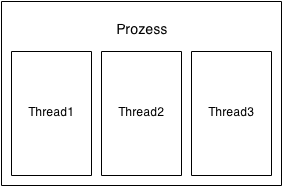
\includegraphics[width=0.3\textwidth]{./data/Threads.png}
	\end{center}
	\vspace{-20pt}
	\caption{Prozess und Threads}
	\vspace{-10pt}
\end{wrapfigure}

\paragraph{Problem:} \\ Die Server-Klasse und Sensor-Klasse befinden sich in einer Endlosschleife, da sie dauerhaft auf eine Eingabe warten. Beim Server sind dies Empfangene Daten und beim Sensor Bewegungssignale. Würden alle Klassen in einem Thread ablaufen, so würde nur eine Klasse gestartet werden und der Anwendungsablauf in dieser bleiben. 
\paragraph{Lösung:} \\ Die beiden oben genannten Klassen, sowie weitere Klassen wie die LED-Steuerung, werden in eigene Threads ausgelagert. Threads sind Unterprozesse im Hauptprozess, die es ermöglichen mehrere Aufgaben in einem Programm gleichzeitig abzuarbeiten. Zwischen den einzelnen Threads kann Datenaustausch statt finden und es ist möglich übergreifende Funktionen aufzurufen. \\
Zur Implementierung wird das Modul 'threading' genutzt. Eine Klasse, die in einem Thread gestartet werden soll, benötigt eine init- und eine run-Methode.
\paragraph{Beispielcode:}\\
Für eine Funktionsdarstellung der Threads mit Python werden drei Klassen angelegt, eine zur Steuerung und zwei, die in einem Thread laufen sollen. \\
Die Klasse 'Testcenter' initialisiert die Klassen als Threads und startet diese.
\begin{lstlisting}[caption=Klasse Testcenter, language=python, frame=single, breaklines=true,columns=fullflexible, commentstyle=\color{gray}\upshape, captionpos=b, numbers = left]
#!/usr/bin/python
# -*- coding: utf-8 -*-
##############################
# Author: Timo Höting                        #
# Mail: mail[at]timohoeting.de            #
##############################
import threading
from TestThread import *
from TestThread1 import *

class TestCenter():
    def newThread(self):
        global testthread
        global testthread1
        testthread = TestThread('thread0', self)
        testthread1 = TestThread1('thread1', self)
        testthread.start()
        testthread1.start()

    def dosth(self):
        print 'dosth'

    def dosth2(self):
        print 'dosth2'

    def dosth3(self):
        testthread1.calledFromMain('-dosth3')

if __name__ == "__main__":
    newThread = TestCenter()
    newThread.newThread()
\end{lstlisting}
Die beiden TestThread-Klassen enthalten beide eine init- und eine run-Methode. Die Klasse Thread1 enthält zusätzlich noch eine Methode die von anderen Klassen ausführbar ist. 
\begin{lstlisting}[caption=Klasse TestThread1, language=python, frame=single, breaklines=true,columns=fullflexible, commentstyle=\color{gray}\upshape, captionpos=b, numbers = left]
#!/usr/bin/python
# -*- coding: utf-8 -*-
##############################
# Author: Timo Höting                        #
# Mail: mail[at]timohoeting.de            #
##############################

import threading
import time
import datetime

class TestThread1(threading.Thread):
    def __init__(self,ms,c):
        threading.Thread.__init__(self)
        global center
        center = c
        global message
        message = ms

    def run(self):
        print message
        center.dosth2()

    def calledFromMain(self, message):
        print  'calledFromMain' + message
\end{lstlisting}
Die init-Methoden werden bei der Erzeugung des Threads aufgerufen und die run-Methode wenn er gestartet wird. Danach können die Methoden wie bei normalen Methodenaufrufen benutzt werden. 